\chapter{Results}
\label{ch:results}

Well over 100 plots, some containing statistical measures, were made for this report.
It is impossible to provide and discuss them all here.
For this reason, we invite the reader to go through the figures and notebooks available on GitHub if any uncertainty would be present \citep{github_project}.
This chapter will discuss how the original paper's results were reproduced and how they are almost identical to the ones obtained using the alternative bark operator.
We also look at a preliminary study on the impact of using a small-community-like network.


%------------------------------------

\section{Reproducing de Boer 2000 and alternative bark operator evaluation}
\label{sec:results_de_boer_bark}

In chapter \ref{ch:reimplementing} we discussed how we re-implemented the imitation games proposed by \citet{deBoer2000}.
Chapter \ref{ch:improving_de_boer} detailed how some of the ad hoc decisions by \citet{deBoer2000} were addressed.
We will discuss the results from experiments performed on these configurations in this section.

While recreating the experiments from \citet{deBoer2000} using the parameters inferred from the paper, we obtained vowel systems that were less tightly clustered than those originally found by \citet{deBoer2000}.
Since we found this difference rather large, we decided to lower the phoneme step size, from 0.1 to 0.025.
This resulted in more tightly clustered vowel systems that also behaved more stable.
The difference of changing this parameter is illustrated in Figure \ref{fig:bdb_smaller_step}.

Next, the emerged vowel systems were analysed by performing imitation games (5000 iterations) over 1000 trials.
The average success rate, vowel system size and energy were calculated.
The found results for both the original ABM and the one using the alternative bark operator are given in figure \ref{fig:general_bark_bdb}.
When comparing the results for the original ABM to the ones obtained by \citet{deBoer2000} we can conclude they are almost identical for the vowel repertoire distribution and the energy distribution.
The success ratio's from our experiments seem to lay a little lower with a peak at 93\% as opposed to almost 100\% with \citet{deBoer2000}.
The latter seems rather unrealistic so we question whether it is a true average over all the played imitation games, both as initiator and imitator.
When comparing the obtained results for the original ABM to that of the alternative bark operator ABM, we can see a lowered average vowel system size.
This was to be expected, as Figure \ref{fig:acoustic_reach} has taught us that the alternative bark operator results in a non-continuous reachable acoustic space that has less reachable area than the original one.
The lower energy for the alternative bark operator is to be expected due to the lower average vowel system size.
Indeed, when a system has fewer vowels, it is easier for it to have more distance between vowels and thus lower average energy.

\clearpage
For both of these ABMs, the effect of the acoustic noise parameter, effective second formant weight and population size were also tested similarly to \citet{deBoer2000}.
The results for the original ABM are nearly identical to those of \citet{deBoer2000} and all of the same conclusions hold.
For these reasons, we won't repeat them here.
The results for the ABM using the alternative bark operator are also in line with the findings of \citet{deBoer2000}.
However, it has to be remembered from our previous finding that the bark operator has a smaller vowel system size on average and thus the found values reflect this.
However, the same conclusions are also applicable for this variant.
In the extra figures list, the results obtained by varying the acoustic noise and effective second formant weight for the ABM using the alternative bark operator are given (Figure \ref{fig:bark_noise_impact} and \ref{fig:bark_weight_impact}).

Lastly, \citet{deBoer2000} compared the found vowel systems to real human vowel systems.
As we lack the linguistic knowledge to perform this analysis, we won't attempt it here.
Figure \ref{fig:overlayed_vowel} shows an overlay of the known vowels with the result of one imitation game.
A linguist might be able to validate its realism from this figure.

\begin{figure*}[ht]
    \centering
    \begin{subfigure}{.30\textwidth}
        \centering
        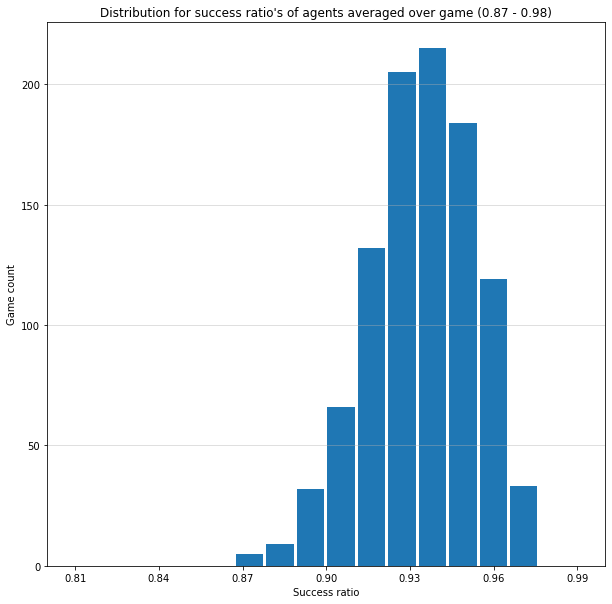
\includegraphics[width=\textwidth]{images/results/original_success.png}
        \captionsetup{width=0.9\linewidth}
        \captionsetup{justification=centering}
        \caption{Average success ratio}
    \end{subfigure}
    \hspace{0.5cm}
    \begin{subfigure}{.30\textwidth}
        \centering
        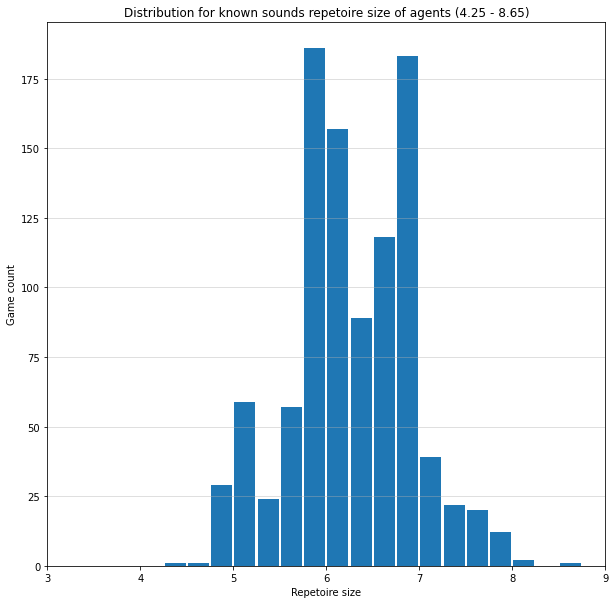
\includegraphics[width=\textwidth]{images/results/original_size.png}
        \captionsetup{width=0.9\linewidth}
        \captionsetup{justification=centering}
        \caption{Average system size}
    \end{subfigure}
    \hspace{0.5cm}
    \begin{subfigure}{.30\textwidth}
        \centering
        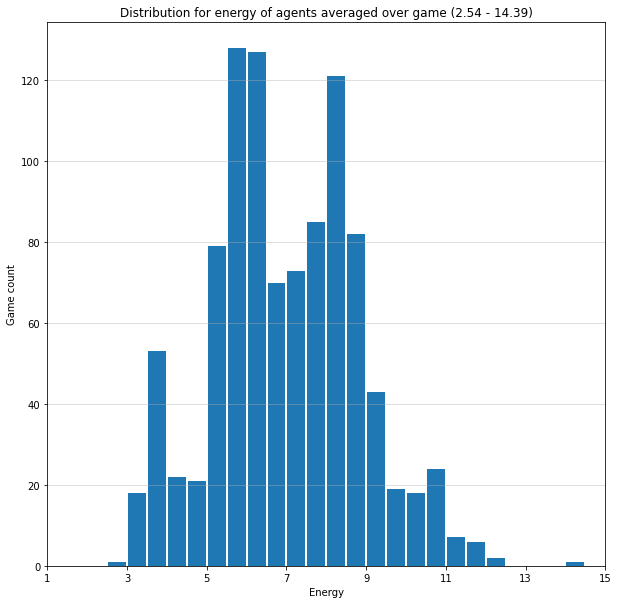
\includegraphics[width=\textwidth]{images/results/original_energy.png}
        \captionsetup{width=0.9\linewidth}
        \captionsetup{justification=centering}
        \caption{Average energy}
    \end{subfigure}
    \begin{subfigure}{.30\textwidth}
        \centering
        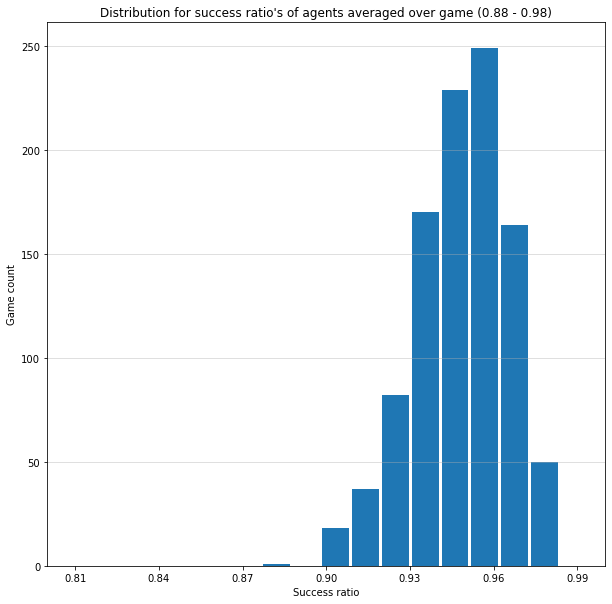
\includegraphics[width=\textwidth]{images/results/bark_sucess.png}
        \captionsetup{width=0.9\linewidth}
        \captionsetup{justification=centering}
        \caption{Average success ratio}
    \end{subfigure}
    \hspace{0.5cm}
    \begin{subfigure}{.30\textwidth}
        \centering
        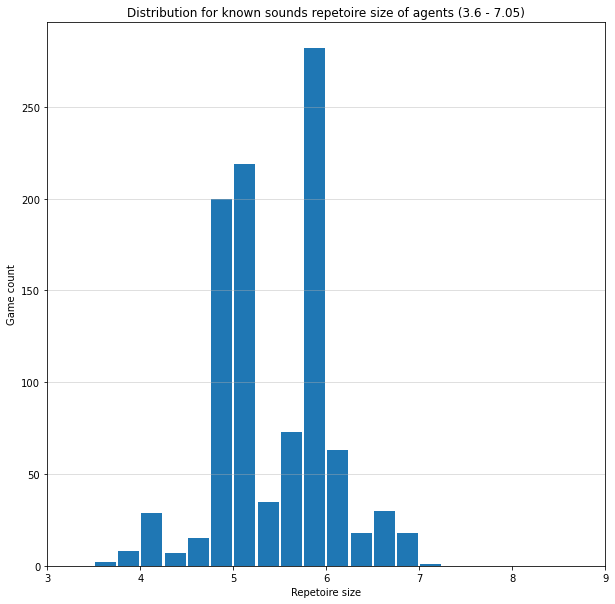
\includegraphics[width=\textwidth]{images/results/bark_size.png}
        \captionsetup{width=0.9\linewidth}
        \captionsetup{justification=centering}
        \caption{Average system size}
    \end{subfigure}
    \hspace{0.5cm}
    \begin{subfigure}{.30\textwidth}
        \centering
        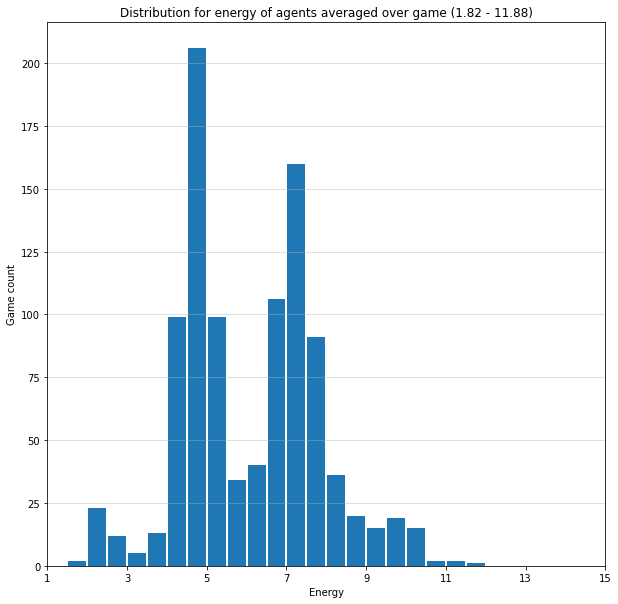
\includegraphics[width=\textwidth]{images/results/bark_energy.png}
        \captionsetup{width=0.9\linewidth}
        \captionsetup{justification=centering}
        \caption{Average energy}
    \end{subfigure}
    \captionsetup{width=0.9\linewidth}
    \captionsetup{justification=centering}
    \caption{Basic statistics of emerged vowel systems averaged over 1000 trials.\\Upper row shows the results from imitation games as described by \citet{deBoer2000}.\\Lower row shows results from using the alternative bark operator.}
    \label{fig:general_bark_bdb}
\end{figure*}


%------------------------------------
\clearpage
\section{preliminary study on the small-community-like network}
\label{sec:results_small_community}

It was originally planned to evaluate the ABM using the small-community-like network discussed in chapter \ref{ch:extension} in an equal manner as the experiments discussed in the previous section.
However, due to limited computational power and a discovery of a bug during the exam sessions, we only were able to perform a preliminary study.
The experiments of this preliminary study already took a combined time of well over 40 computer hours to complete.

Figure \ref{fig:samples_community} shows an example of the vowel systems that emerge from this ABM.
This plot shows 2 different configurations.
The top row shows a configuration where 8000 iterations were played and a generation change (shift up) happened after the 4000th iteration.
Although having only 2 generations, it can be considered a vertical ABM.
The bottom row shows a similar configuration but without a generation shift, only a transition from babies to students after the 4000th iteration.
This system reflects a horizontal ABM such as the one used by \citet{deBoer2000}.
Both show the same emergent effect observed previously.
The non-generational variant appears to have more clusters on average than the generational one, which is expected to be caused by the generation shift.
More interestingly, when looking at the plot of only highly educated agents (doctorates and professors) we can see the clusters are very tight compared to those of the regularly educated agents (parents and grandparents) and seen in the all agents plot.



\begin{figure*}[ht]
    \centering
    \begin{subfigure}{.30\textwidth}
        \centering
        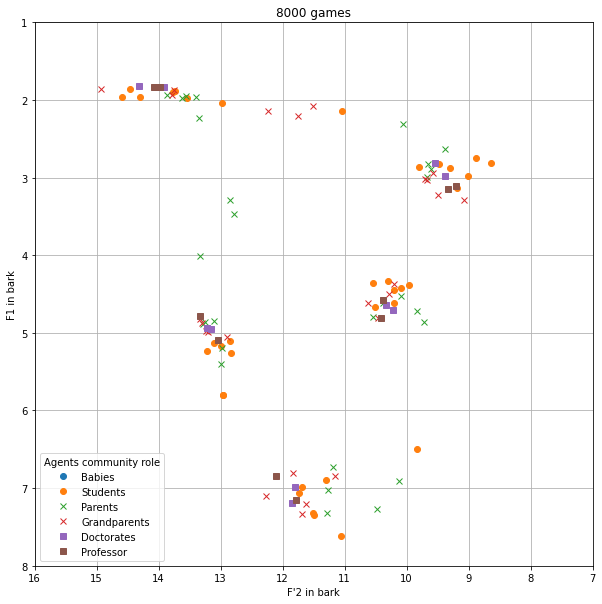
\includegraphics[width=\textwidth]{images/results/dual_all.png}
        \captionsetup{width=0.9\linewidth}
        \captionsetup{justification=centering}
        \caption{All agents}
    \end{subfigure}
    \hspace{0.5cm}
    \begin{subfigure}{.30\textwidth}
        \centering
        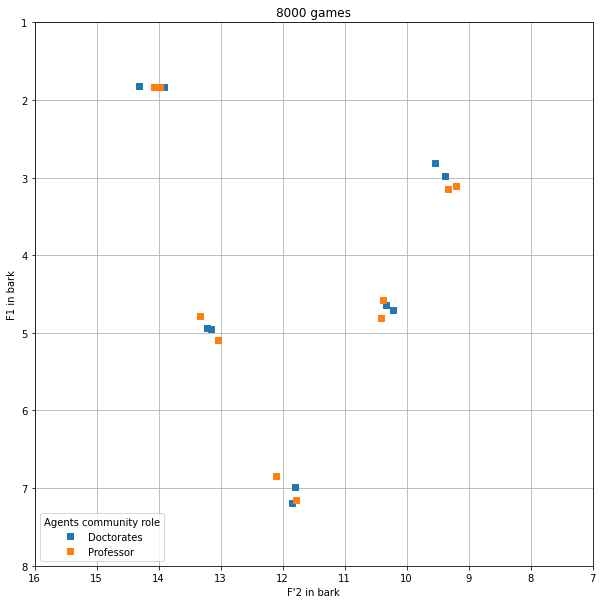
\includegraphics[width=\textwidth]{images/results/dual_high.png}
        \captionsetup{width=0.9\linewidth}
        \captionsetup{justification=centering}
        \caption{Highly educated agents}
    \end{subfigure}
    \hspace{0.5cm}
    \begin{subfigure}{.30\textwidth}
        \centering
        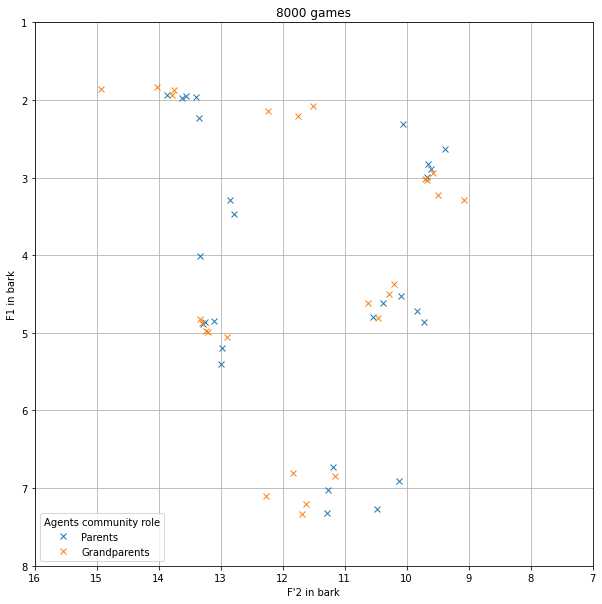
\includegraphics[width=\textwidth]{images/results/dual_regular.png}
        \captionsetup{width=0.9\linewidth}
        \captionsetup{justification=centering}
        \caption{Regular educated agents}
    \end{subfigure}
    \begin{subfigure}{.30\textwidth}
        \centering
        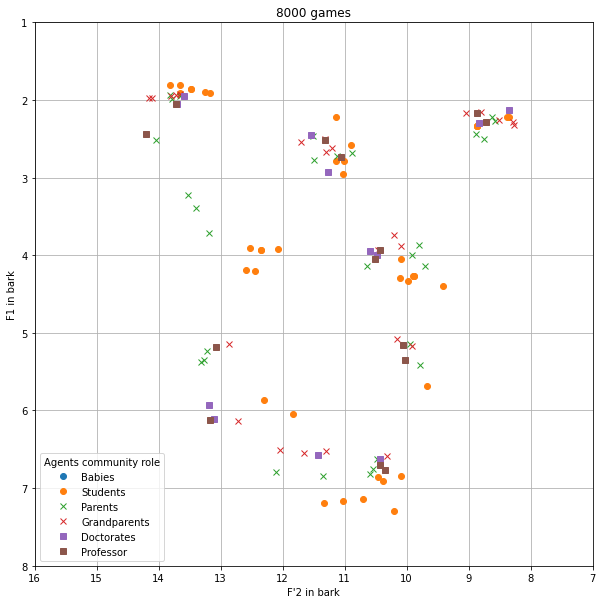
\includegraphics[width=\textwidth]{images/results/singla_all.png}
        \captionsetup{width=0.9\linewidth}
        \captionsetup{justification=centering}
        \caption{All agents}
    \end{subfigure}
    \hspace{0.5cm}
    \begin{subfigure}{.30\textwidth}
        \centering
        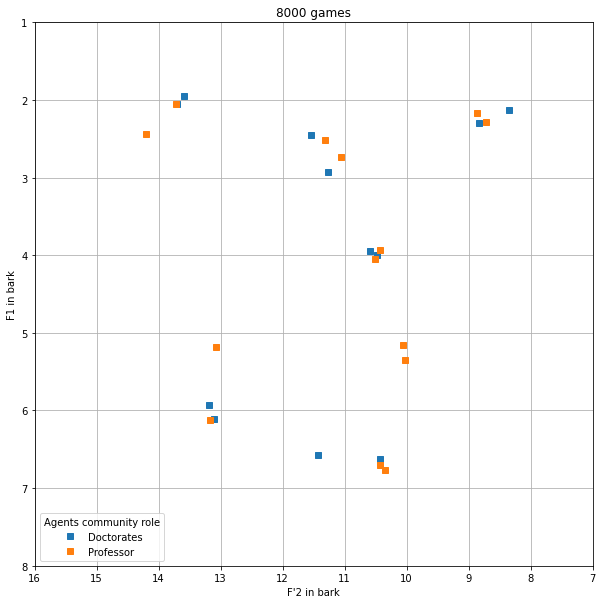
\includegraphics[width=\textwidth]{images/results/single_high.png}
        \captionsetup{width=0.9\linewidth}
        \captionsetup{justification=centering}
        \caption{Highly educated agents}
    \end{subfigure}
    \hspace{0.5cm}
    \begin{subfigure}{.30\textwidth}
        \centering
        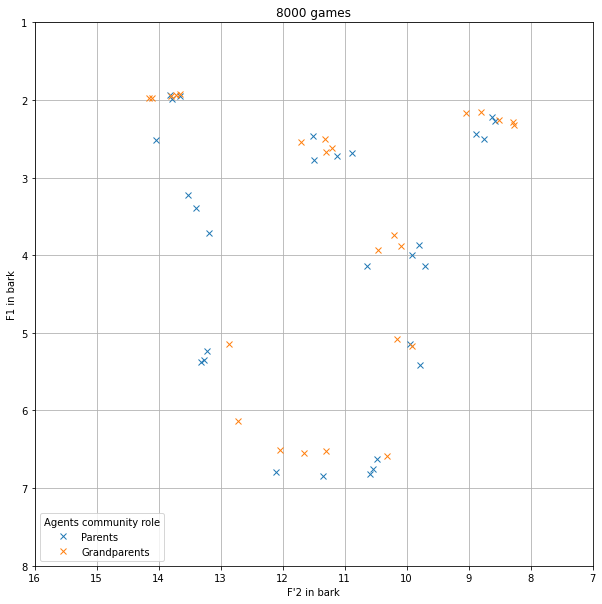
\includegraphics[width=\textwidth]{images/results/single_regular.png}
        \captionsetup{width=0.9\linewidth}
        \captionsetup{justification=centering}
        \caption{Regular educated agents}
    \end{subfigure}
    \captionsetup{width=0.9\linewidth}
    \captionsetup{justification=centering}
    \caption{Example vowel system emerged from ABM using the custom network.\\Upper row shows results for an imitation game using multiple generations.\\Lower row shows results from using a fixed generation.}
    \label{fig:samples_community}
\end{figure*}


\clearpage
Just as before, the average success rate, vowel system size and energy were calculated.
This was done using 6000 iteration games with a generation shift at the 4000th iteration.
The average was taken over 100 trials.
When studying these metrics for all agents, we get a wrong view of the reality as the distributions of these metrics are different for students, highly educated agents and regularly educated agents.
An overview of these metrics for all agents, the highly educated ones and the regularly educated ones is given in Figure \ref{fig:general_community}.

Most interestingly is the fact that the highly educated agents have an average vowel system size of 5.6 with a standard deviation of 1.7.
This seems to lie higher compared to the average vowel system size of 4.2 with a standard deviation of 1 for the regular educated agents.
However, due to the large standard deviations, we can't conclude there is a statistically significant difference.
Ideally, this experiment would be re-performed over more iterations and trials to obtain better statistics.

Lastly, an experiment was performed to test the impact of the acoustic noise parameter on the found vowel systems.
This is done by comparing the network configured as before but using the original acoustic noise settings, double the acoustic noise and triple the acoustic noise.
An overview of the results is given in Figure \ref{fig:noise_community}.
As was the case for the experiments by \citet{deBoer2000}, the average vowel system size decreases as noise increases.
In higher noise conditions the fitness advantage of highly educated agents also becomes more obvious.
Again, the iteration amount of these experiments and perhaps the trial amount should be increased to make statistical concussions possible.



\begin{figure*}[ht]
    \centering
    \begin{subfigure}{.30\textwidth}
        \centering
        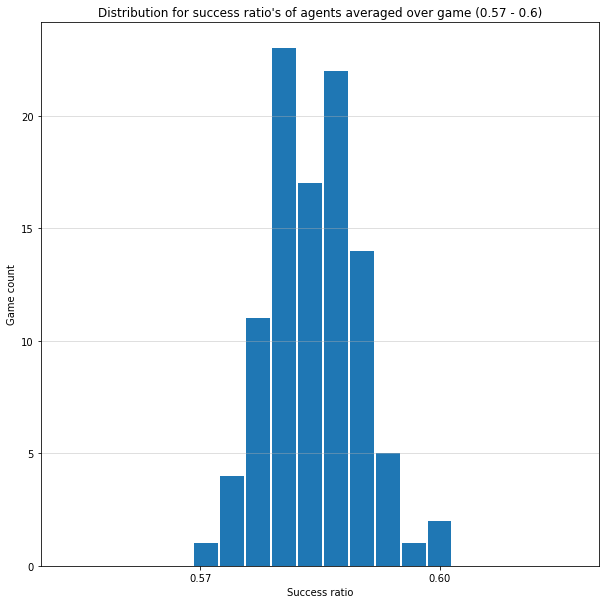
\includegraphics[width=\textwidth]{images/results/all_success.png}
        \captionsetup{width=0.9\linewidth}
        \captionsetup{justification=centering}
        \caption{Average success ratio}
    \end{subfigure}
    \hspace{0.5cm}
    \begin{subfigure}{.30\textwidth}
        \centering
        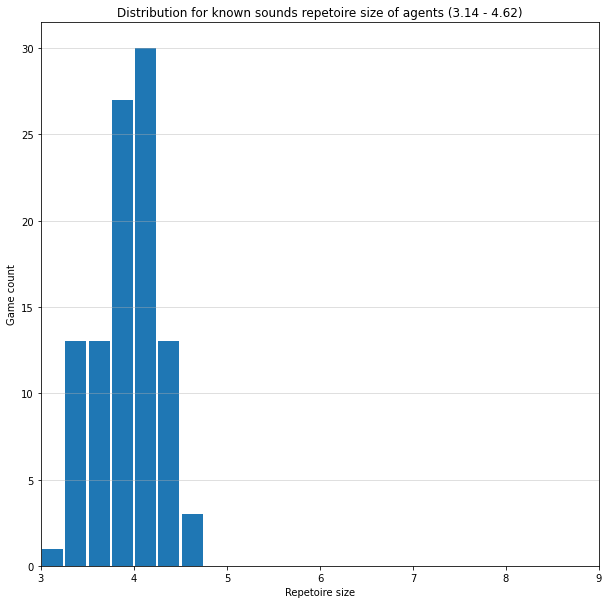
\includegraphics[width=\textwidth]{images/results/all_size.png}
        \captionsetup{width=0.9\linewidth}
        \captionsetup{justification=centering}
        \caption{average system size}
    \end{subfigure}
    \hspace{0.5cm}
    \begin{subfigure}{.30\textwidth}
        \centering
        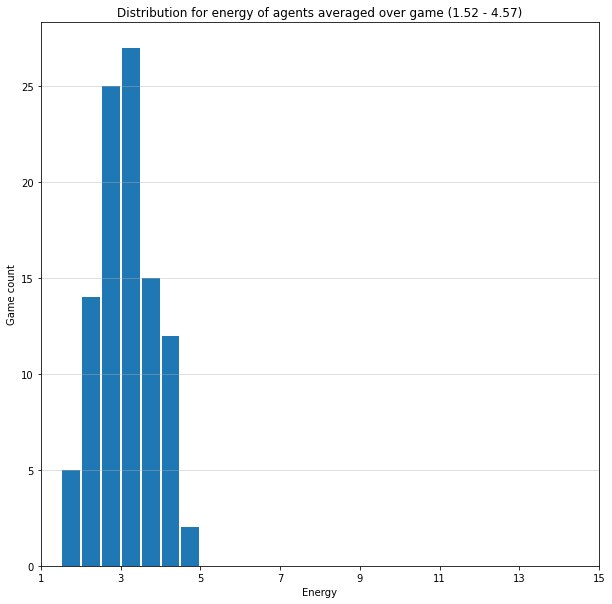
\includegraphics[width=\textwidth]{images/results/all_energy.png}
        \captionsetup{width=0.9\linewidth}
        \captionsetup{justification=centering}
        \caption{Average energy}
    \end{subfigure}
    \begin{subfigure}{.30\textwidth}
        \centering
        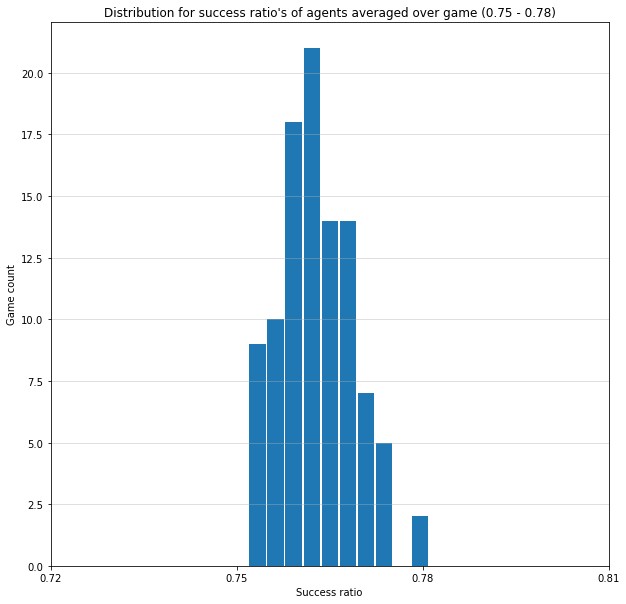
\includegraphics[width=\textwidth]{images/results/high_success.png}
        \captionsetup{width=0.9\linewidth}
        \captionsetup{justification=centering}
        \caption{Average success ratio}
    \end{subfigure}
    \hspace{0.5cm}
    \begin{subfigure}{.30\textwidth}
        \centering
        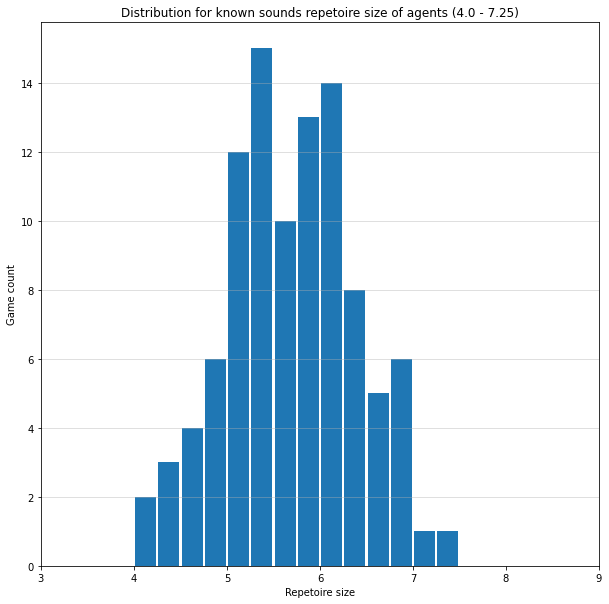
\includegraphics[width=\textwidth]{images/results/high_size.png}
        \captionsetup{width=0.9\linewidth}
        \captionsetup{justification=centering}
        \caption{average system size}
    \end{subfigure}
    \hspace{0.5cm}
    \begin{subfigure}{.30\textwidth}
        \centering
        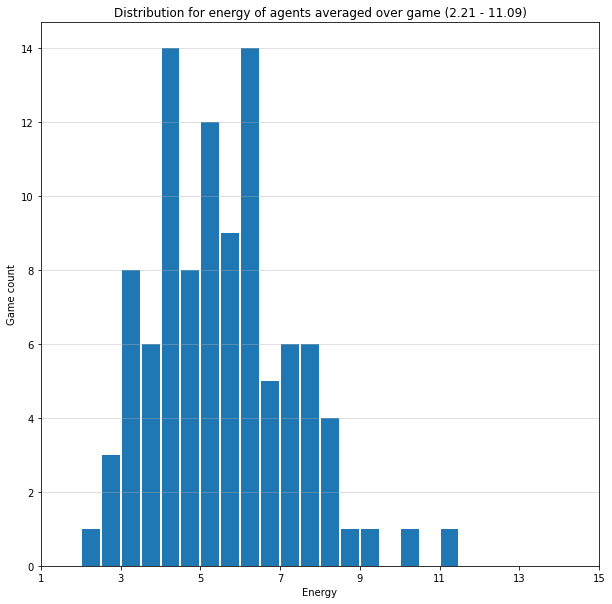
\includegraphics[width=\textwidth]{images/results/high_energy.png}
        \captionsetup{width=0.9\linewidth}
        \captionsetup{justification=centering}
        \caption{Average energy}
    \end{subfigure}
    \begin{subfigure}{.30\textwidth}
        \centering
        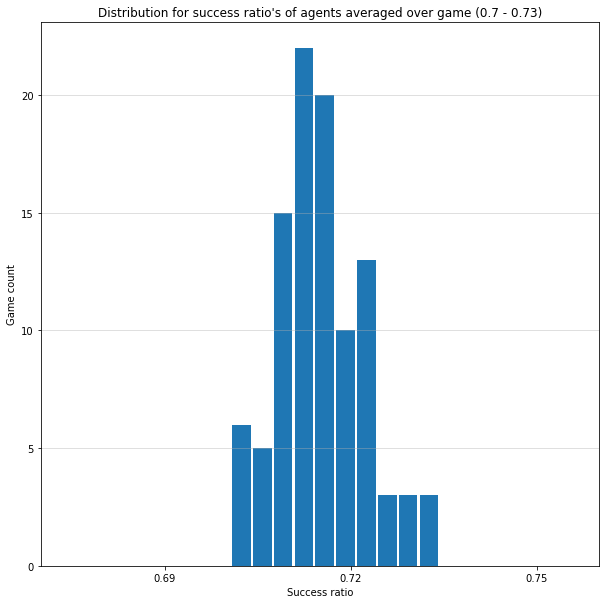
\includegraphics[width=\textwidth]{images/results/regular_success.png}
        \captionsetup{width=0.9\linewidth}
        \captionsetup{justification=centering}
        \caption{Average success ratio}
    \end{subfigure}
    \hspace{0.5cm}
    \begin{subfigure}{.30\textwidth}
        \centering
        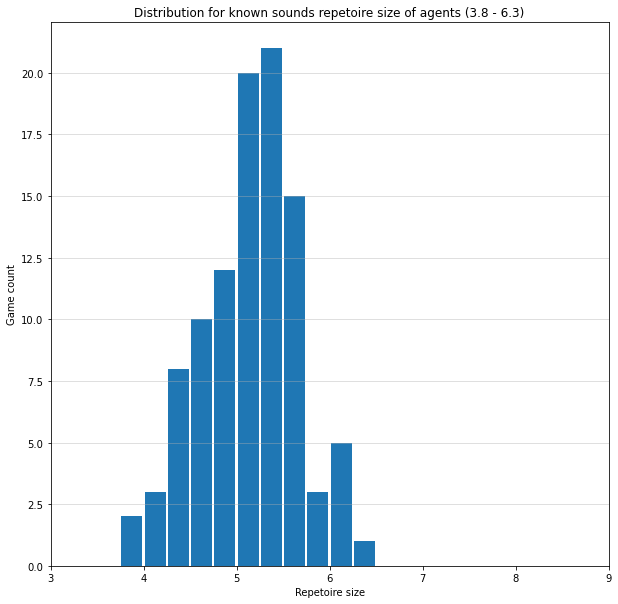
\includegraphics[width=\textwidth]{images/results/regular_size.png}
        \captionsetup{width=0.9\linewidth}
        \captionsetup{justification=centering}
        \caption{average system size}
    \end{subfigure}
    \hspace{0.5cm}
    \begin{subfigure}{.30\textwidth}
        \centering
        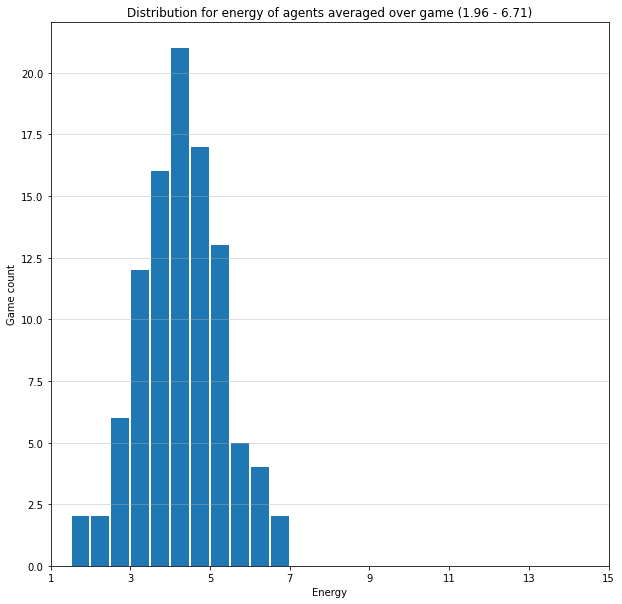
\includegraphics[width=\textwidth]{images/results/regular_energy.png}
        \captionsetup{width=0.9\linewidth}
        \captionsetup{justification=centering}
        \caption{Average energy}
    \end{subfigure}
    \captionsetup{width=\linewidth}
    \captionsetup{justification=centering}
    \caption{Basic statistics of emerged vowel systems averaged over 100 trials.
    \\Upper row shows the results for all agents in a custom network ABM.
    \\Middle row shows the results for highly educated agents in a custom network ABM.
    \\Bottom row shows the results for regularly educated agents in a custom network ABM.
    \\Note that the scale for the success distribution differs between rows.}
    \label{fig:general_community}
\end{figure*}

%-------------------------------------------




\begin{figure*}[ht]
    \centering
    \begin{subfigure}{.30\textwidth}
        \centering
        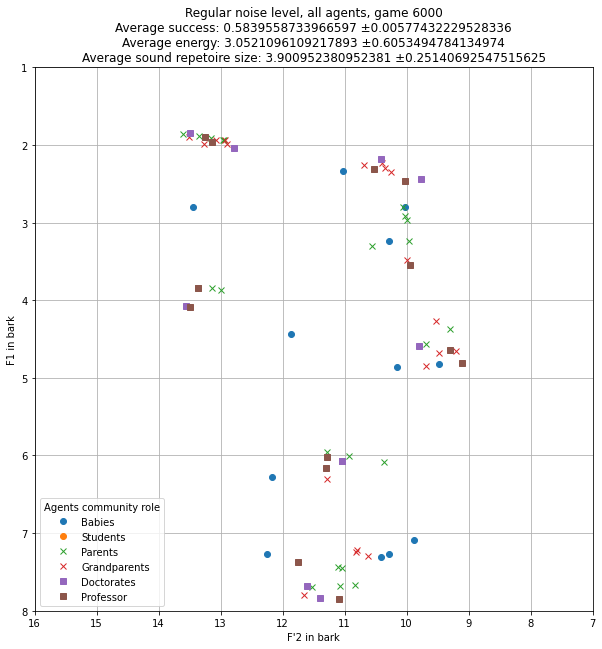
\includegraphics[width=\textwidth]{images/results/noise_std_all.png}
        \captionsetup{width=0.9\linewidth}
        \captionsetup{justification=centering}
        \caption{All agents}
    \end{subfigure}
    \hspace{0.5cm}
    \begin{subfigure}{.30\textwidth}
        \centering
        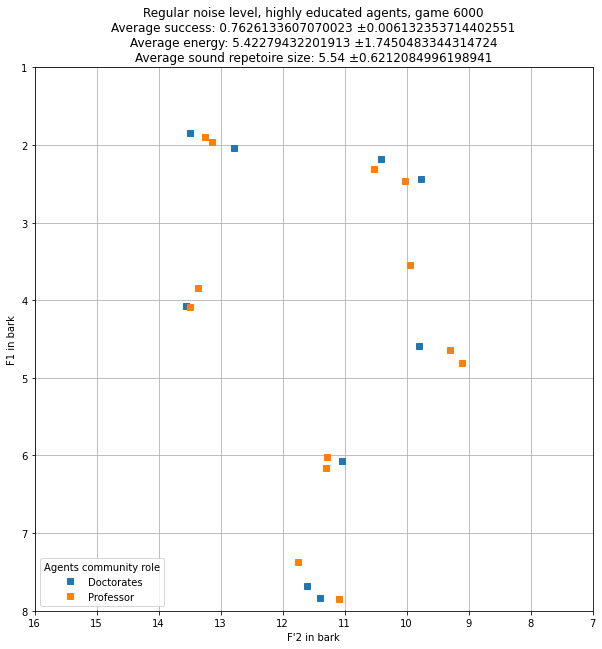
\includegraphics[width=\textwidth]{images/results/noise_std_high.png}
        \captionsetup{width=0.9\linewidth}
        \captionsetup{justification=centering}
        \caption{Highly educated agents}
    \end{subfigure}
    \hspace{0.5cm}
    \begin{subfigure}{.30\textwidth}
        \centering
        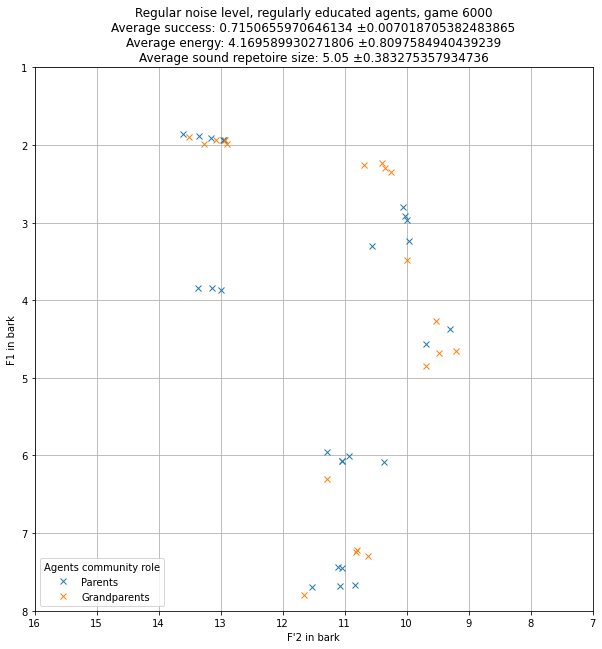
\includegraphics[width=\textwidth]{images/results/noise_std_regular.png}
        \captionsetup{width=0.9\linewidth}
        \captionsetup{justification=centering}
        \caption{Regular educated agents}
    \end{subfigure}
    \begin{subfigure}{.30\textwidth}
        \centering
        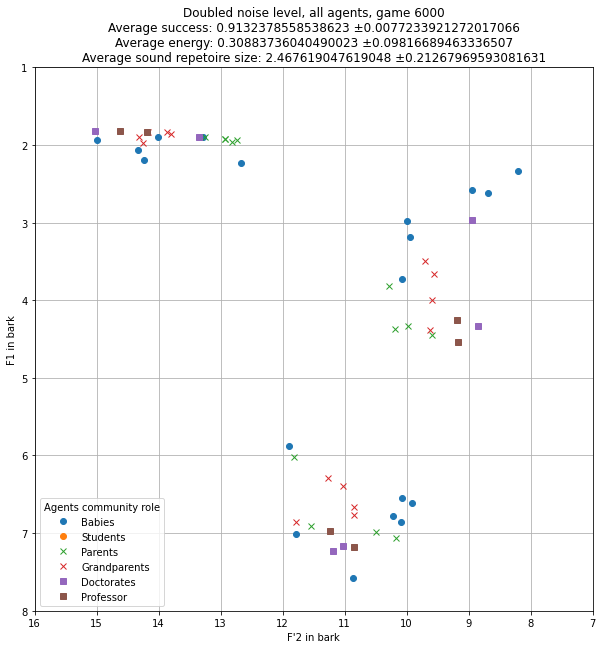
\includegraphics[width=\textwidth]{images/results/double_noise_all.png}
        \captionsetup{width=0.9\linewidth}
        \captionsetup{justification=centering}
        \caption{All agents}
    \end{subfigure}
    \hspace{0.5cm}
    \begin{subfigure}{.30\textwidth}
        \centering
        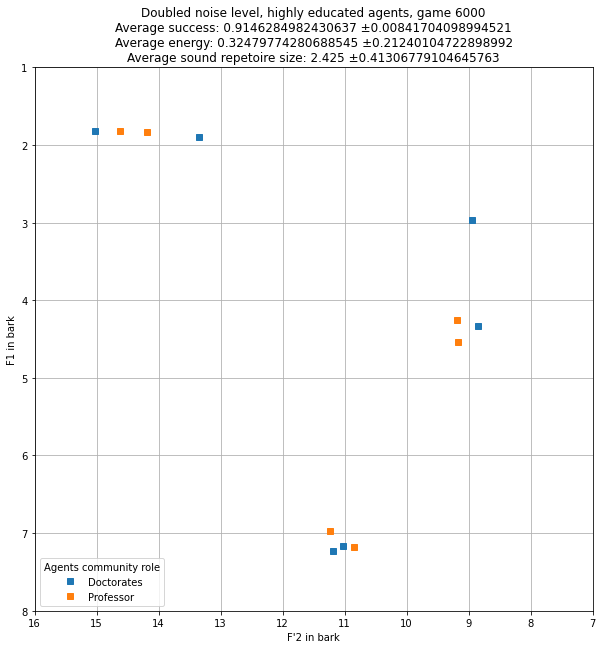
\includegraphics[width=\textwidth]{images/results/double_noise_high.png}
        \captionsetup{width=0.9\linewidth}
        \captionsetup{justification=centering}
        \caption{Highly educated agents}
    \end{subfigure}
    \hspace{0.5cm}
    \begin{subfigure}{.30\textwidth}
        \centering
        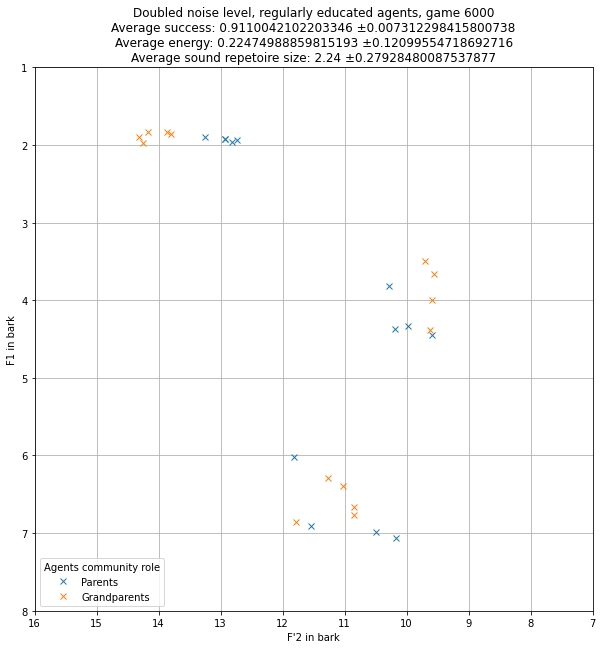
\includegraphics[width=\textwidth]{images/results/double_noise_regular.png}
        \captionsetup{width=0.9\linewidth}
        \captionsetup{justification=centering}
        \caption{Regular educated agents}
    \end{subfigure}
    \begin{subfigure}{.30\textwidth}
        \centering
        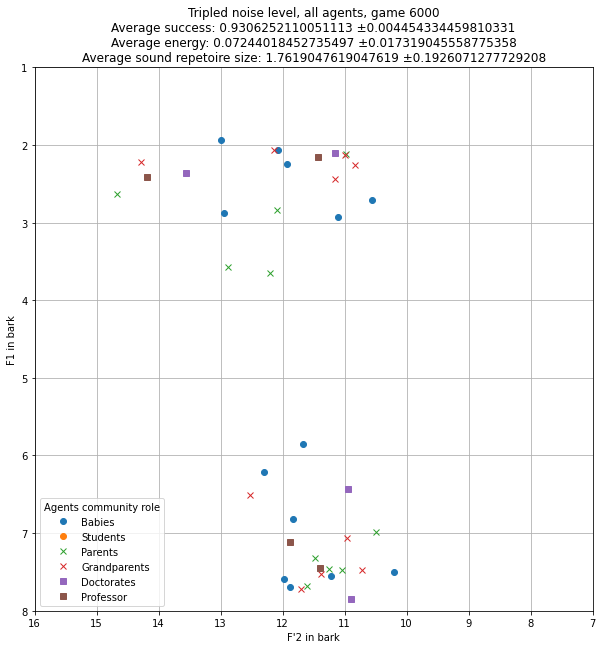
\includegraphics[width=\textwidth]{images/results/triple_noise_all.png}
        \captionsetup{width=0.9\linewidth}
        \captionsetup{justification=centering}
        \caption{All agents}
    \end{subfigure}
    \hspace{0.5cm}
    \begin{subfigure}{.30\textwidth}
        \centering
        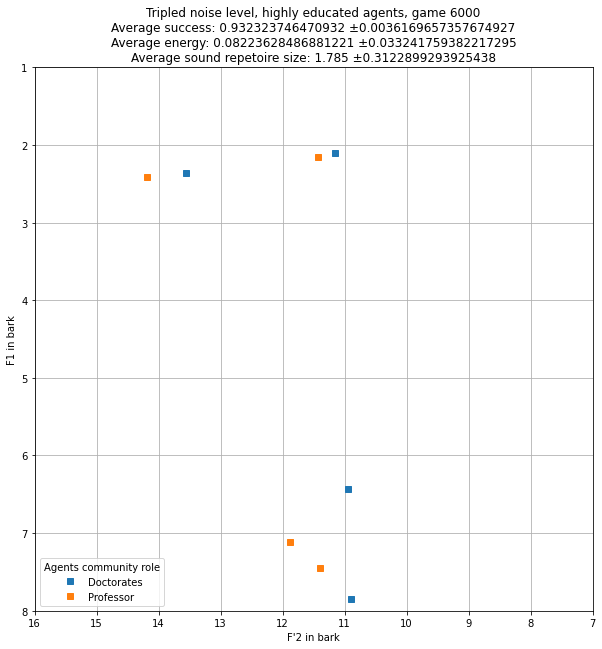
\includegraphics[width=\textwidth]{images/results/triple_noise_high.png}
        \captionsetup{width=0.9\linewidth}
        \captionsetup{justification=centering}
        \caption{Highly educated agents}
    \end{subfigure}
    \hspace{0.5cm}
    \begin{subfigure}{.30\textwidth}
        \centering
        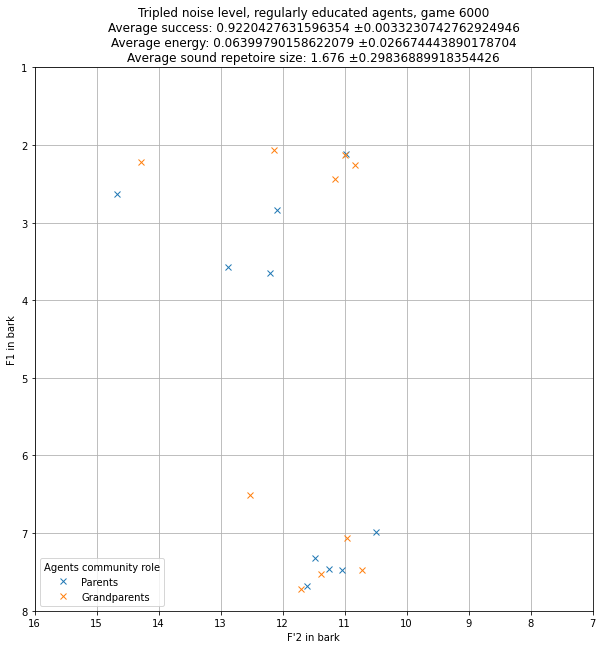
\includegraphics[width=\textwidth]{images/results/triple_noise_regular.png}
        \captionsetup{width=0.9\linewidth}
        \captionsetup{justification=centering}
        \caption{Regular educated agents}
    \end{subfigure}
    \captionsetup{width=\linewidth}
    \captionsetup{justification=centering}
    \caption{Example plot of vowel systems in different acoustic noise settings.
    \\ Statistics above plot are averaged over 50 trials.
    \\Upper row shows the results of regular noise in a custom network ABM.
    \\Midlle row shows the results of doubled noise in a custom network ABM.
    \\Lower row shows the results of tripled noise in a custom network ABM.}
    \label{fig:noise_community}
\end{figure*}